\section{Sensorik}
\label{Sensorik_secd}
Die Aufgabe der verwendeten Sensorik liegt darin die Werte für $\varphi$, und $\dot{\varphi}$ zu bestimmen. Hierfür wurden zwei MPU6050 IC's verwendet. Diese verfügen jeweils über einen Beschleunigungssensor und Gyroskop, welche Werte für drei Achsen ausgeben. Der Tiefpass der Sensoren wird auf eine Grenzfrequenz von $44Hz$ eingestellt, da hier einerseits eine erste Glättung der Daten erfolgt, andererseits aber keine zu große Verzögerung ergibt, welche sich wiederum negativ auf die Regelung auswirken könnte. Die Position und Ausrichtung der Sensoren ist in \ref{Position_Sensoren_pic} dargestellt.

\begin{figure}[h]
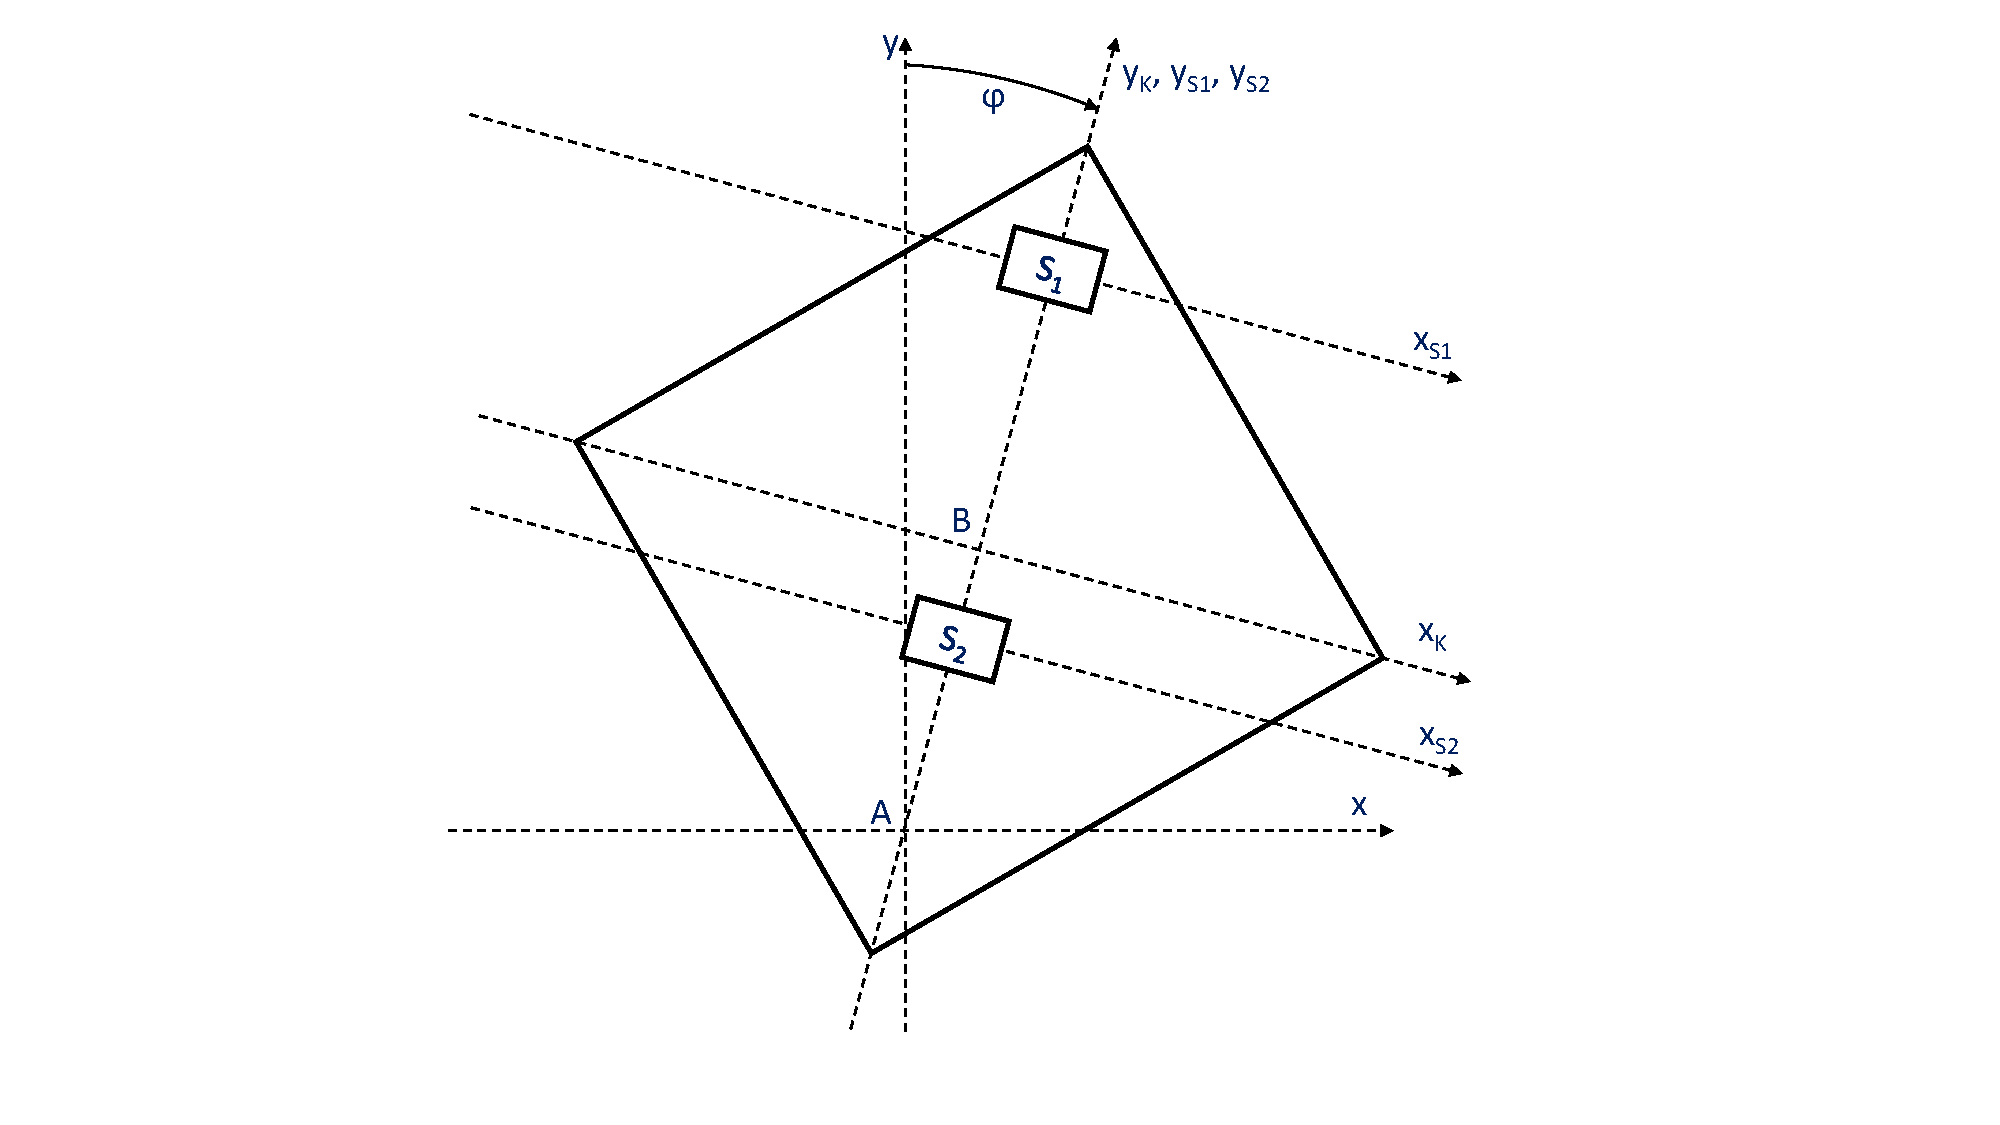
\includegraphics[width=\linewidth]{SensorZeichnung1D}
\caption{Position der Sensoren, Quelle: eigene Darstellung}

\label{Position_Sensoren_pic}
\end{figure}

\subsection{Winkelschätzung}
Die Sensoren keine Wege bzw. Winkel. Somit muss der Winkel $\varphi$ berechnet werden. Die gemessenen Sensorwerte hängen von $r_{S1}$ bzw. $r_{S2}$ ab, welche den Abstand zwischen den Sensoren und dem Drehpunkt $A$ beschreiben. Zusätzlich beeinflussen neben dem Winkel $\varphi$ auch dessen beiden Ableitungen $\dot{\varphi}$ und $\ddot{\varphi}$ die Sensorausgabe. Allerdings lassen sich aus den Beschleunigungswerten der beiden Sensoren nach \cite{Cubli1D} wie folgt der aktuelle Wert von $\varphi$ berechnen.

\begin{equation}
\ddot{S}_i = 
\begin{pmatrix}
\ddot{x}_i \\ \ddot{y}_i \\ \ddot{z}_i
\end{pmatrix} =
\begin{pmatrix}
r_{Si} \cdot \ddot{\varphi} + sin(\varphi) \cdot g \\
- r_{Si} \cdot \dot{\varphi}^2 - cos(\varphi) \cdot g \\
0
\end{pmatrix}
\hspace{35pt}
i \in [1;2]
\end{equation}

\begin{equation}
\alpha = \frac{r_{S1}}{r_{S2}}
\end{equation}

\begin{equation}
\ddot{x}_1 - \alpha \cdot \ddot{x}_2 = 
g(1 - \alpha)sin(\varphi)
\end{equation}
\begin{equation}
\ddot{y}_1 - \alpha \cdot \ddot{y}_2 = 
-g(1- \alpha)cos(\varphi)
\end{equation}

\begin{equation}
\frac{\ddot{x}_1 - \alpha \cdot \ddot{x}_2}{\ddot{y}_1 - \alpha \cdot \ddot{y}_2} = -tan(\varphi)
\end{equation}

\subsection{Kalibrierung und Justierung}
Die Sensoren geben die Beschleunigungs- und Geschwindigkeitswerte als 16 Bit Werte im Zweierkomplement aus. Diese Rohwerte müssen in die mit Hilfe eines Ausgleichspolynoms in die jeweilige SI-Einheit umgerechnet werden. 

\subsubsection{Umrechnung der Beschleunigungswerte}
Um das Polynom zur Umrechnung der Beschleunigungswerte zu ermitteln werden sieben Messungen in den fixen Ausfallpositionen $\phi \in [-45, -30, -15, 0, 15, 30, 45]$ durchgeführt. Pro Position werden $m = 10000$ Messwerte aufgenommen. Da in der Ruhelage die Beschleunigung lediglich von dem aktuellen Ausfallwinkel abhängt ist der Sollwert für jede Position bekannt. Somit kann ein Polynom erster Ordnung approximiert werden um Mittelwerte der sieben Positionen in die entsprechenden Beschleunigungswerte umzurechnen.

\begin{table}[h]
\centering
\begin{tabular}{lcllcl}
$\ddot{x}_n$ &$\equiv$& X-Beschleunigung Sensor n &
$\ddot{x}^R_n$ &$\equiv$& X-Rohwert Sensor n \\
$\ddot{y}_n$ &$\equiv$& Y-Beschleunigung Sensor n &
$\ddot{y}^R_n$ &$\equiv$& Y-Rohwert Sensor n
\end{tabular}
\end{table}

\vspace*{-\baselineskip}
\begin{equation}
\ddot{x}_n = p^1_{x_n} \cdot \ddot{x}^R_n + p^2_{x_n} \hspace{35pt} \vert \hspace{3pt} n \in \{1, 2\}
\end{equation}
\begin{equation}
\ddot{y}_n = p^1_{y_n} \cdot \ddot{y}^R_n + p^2_{y_n} \hspace{35pt} \vert \hspace{3pt} n \in \{1, 2\}
\end{equation}
\vspace*{-\baselineskip}
\begin{table}[h]
\centering
\begin{tabular}{lcllcl}
$p^1_{x_1}$ &$=$& $-6.082 \cdot 10^{-4}$ & $p^2_{x_1}$ &$=$& $0.4412$ \\
$p^1_{x_2}$ &$=$& $-6.07 \cdot 10^{-4}$ & $p^2_{x_2}$ &$=$& $0.2804$ \\
$p^1_{y_1}$ &$=$& $-6.064 \cdot 10^{-4}$ & $p^2_{y_1}$ &$=$& $0.1248$ \\
$p^1_{y_2}$ &$=$& $-6.089 \cdot 10^{-4}$ & $p^2_{y_2}$ &$=$& $0.09182$ \\
\end{tabular}
\end{table}

\vspace*{-\baselineskip}
\begin{figure}[h]
	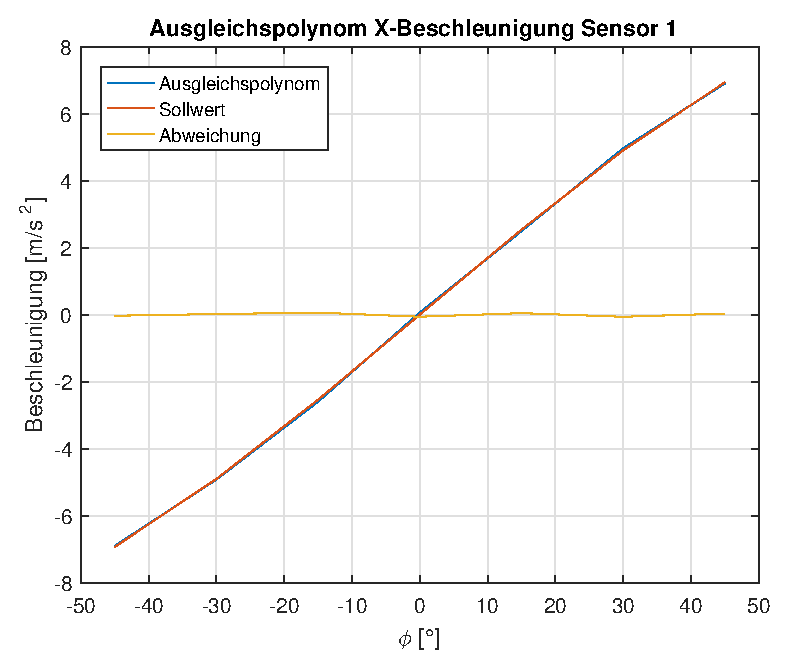
\includegraphics[width=0.5\linewidth]{img/X1__dd___fitted.eps}
	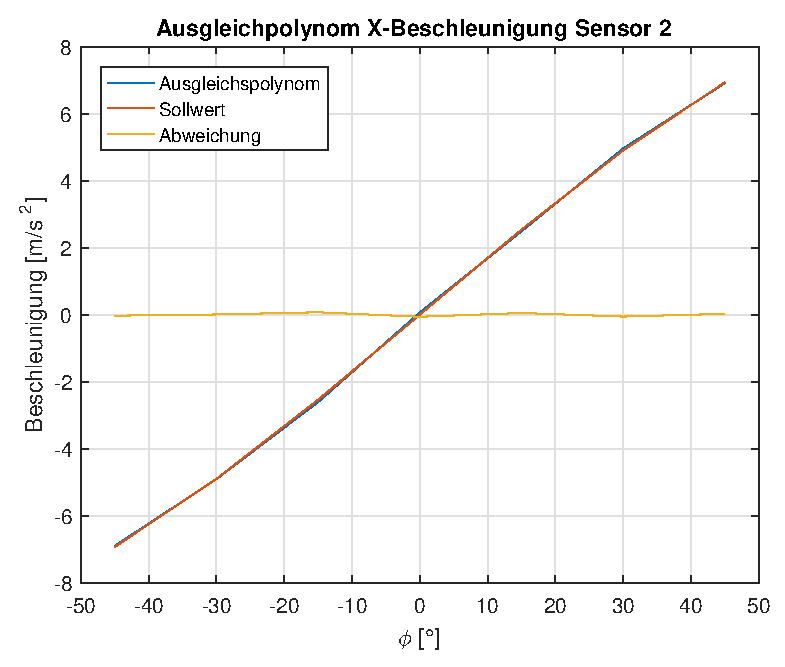
\includegraphics[width=0.5\linewidth]{img/X2__dd___fitted.eps}
\end{figure}

\vspace*{-\baselineskip}
\begin{figure}[h!]
	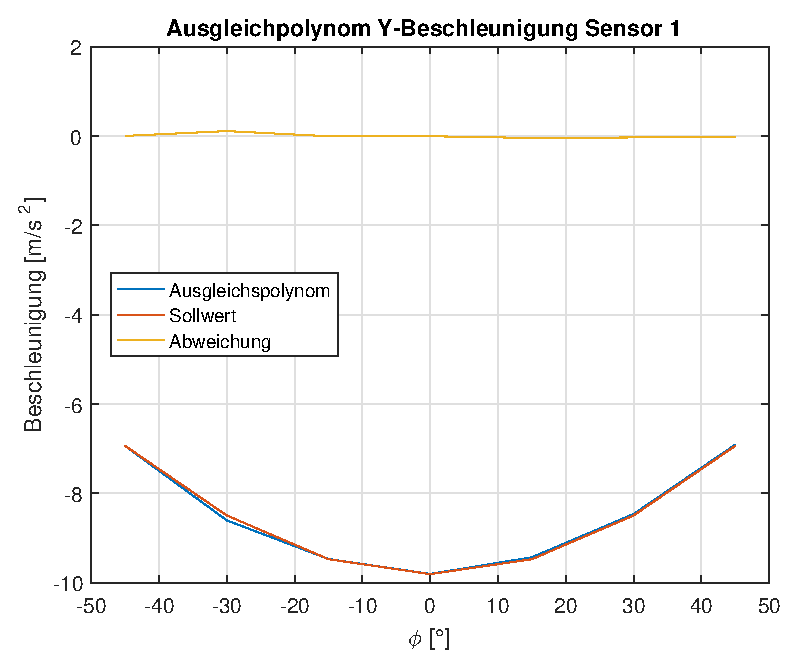
\includegraphics[width=0.5\linewidth]{img/Y1__dd___fitted.eps}
	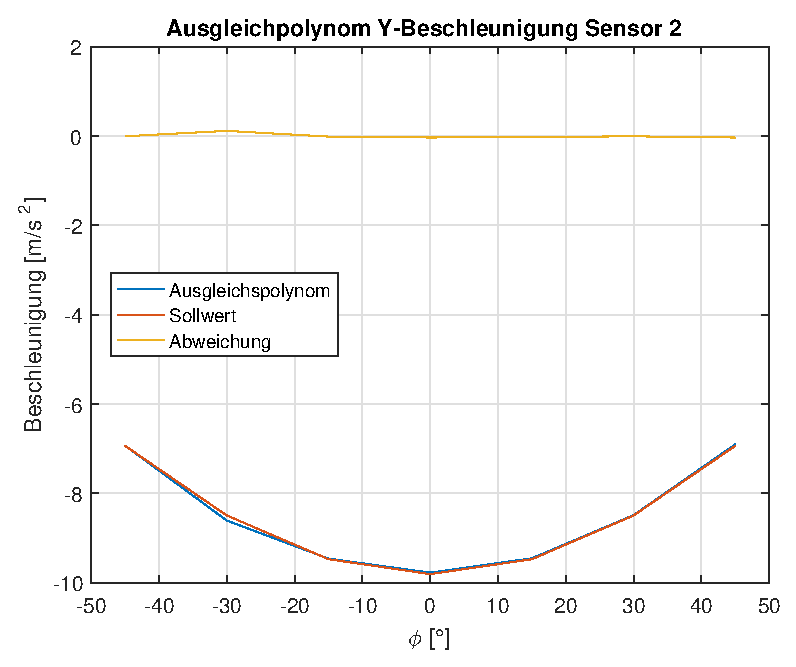
\includegraphics[width=0.5\linewidth]{img/Y2__dd___fitted.eps}
\end{figure}

\subsubsection{Umrechnung der Winkelgeschwindigkeiten}
Um die Rohwerte der Gyroskope in Winkelgeschwindigkeiten umzurechnen wird die Würfelseite fixiert und die Winkelgeschwindigkeitswerte der beiden Sensoren aufgenommen. Hierbei werden jeweils $m = 1000$ Werte aufgenommen. Da der Sollwert $\dot{\varphi} = 0 \frac{m}{s}$ bekannt ist kann die systematische Messabweichung der Sensoren über den Mittelwert bestimmt werden. Der proportionale Umrechnungsfaktor von Rohdaten zu Winkelgeschwindigkeiten wird dem Datenblatt des Herstellers entnommen.

\begin{figure}[h]
	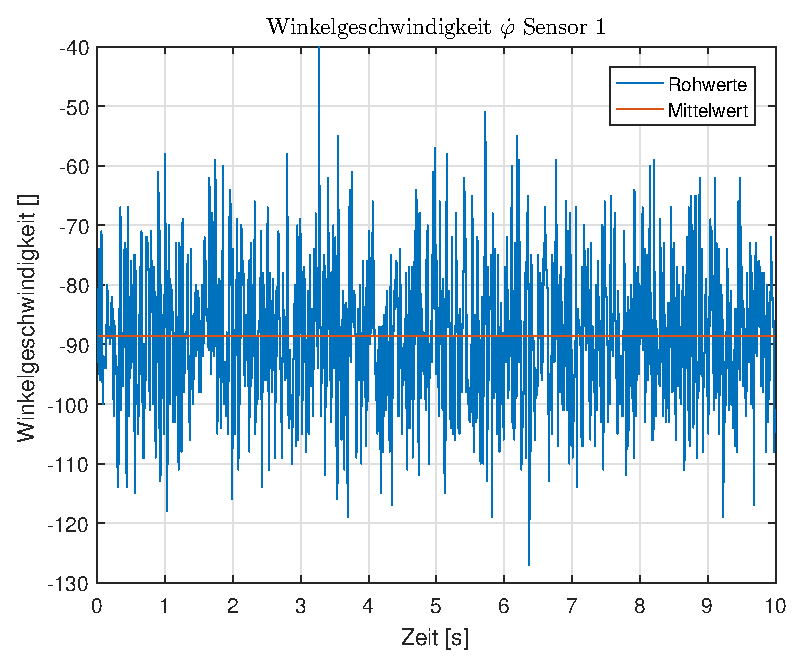
\includegraphics[width=0.5\linewidth]{img/phi1__d.eps}
	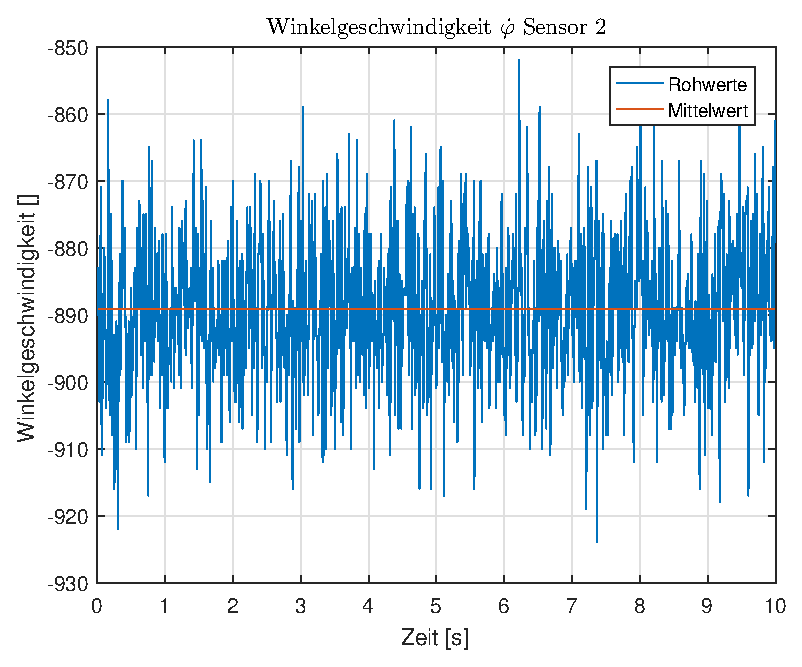
\includegraphics[width=0.5\linewidth]{img/phi2__d.eps}
\end{figure}

\begin{table}[h]
\centering
\begin{tabular}{lcllcl}
$\dot{\varphi}_n$ & $\equiv$ & $\varphi$-Geschwindigkeit Sensor n & $\dot{\varphi}^R_n$ & $\equiv$ $\dot{\varphi}$-Rohwert Sensor n
\end{tabular}
\end{table}

\begin{equation}
\dot{\varphi}_n = p^1_{\dot{\varphi}^R_n}  \cdot (\dot{\varphi}_n + p^2_{\dot{\varphi}_n})
\end{equation}

\begin{table}[h]
\centering
\begin{tabular}{lcllcl}
$p^1_{\varphi_1}$ &$=$& $-0.0076$ & $p^2_{\varphi_1}$ &$=$& $89$ \\
$p^1_{\varphi_2}$ &$=$& $-0.0076$ & $p^2_{\varphi_2}$ &$=$& $889$ \\
\end{tabular}
\end{table}

\subsection{Auswertung der Radgeschwindigkeit $\dot{\psi}$}
Der Motortreiber liefert ein analoges Spannungssignal, welches die aktuelle Motorgeschwindigkeit wiedergibt. Um die ADC-Werte in SI-Einheiten umzurechnen wird ein Polynom erster Ordnung benötigt. Hierfür werden mit Hilfe der ESCON-Studio konstante Motorgeschwindigkeiten ($\dot{\psi} \in \{ -3000, -2000,$  $-1000, 0, 1000, 2000, 3000 \} [rpm] $) gefahren und pro Durchlauf $m=500$ ADC-Werte aufgenommen. Über die Mittelwerte der Messungen und die vorgegebenen Radgeschwindigkeiten wird anschließend ein Polynom erster Ordnung approximiert.

\begin{table}[h!]
\centering
\begin{tabular}{lcllcl}
$\dot{\psi}$ & $\equiv$ & Geschwindigkeit der Schwungmasse & $\dot{\psi}_{ADC}$ & $\equiv$ & ADC-Wert
\end{tabular}
\end{table}

\begin{equation}
\dot{\psi} = -0.5176 \cdot \dot{\psi}_{ADC} + 1017
\end{equation}

\begin{figure}[h!]
\centering
	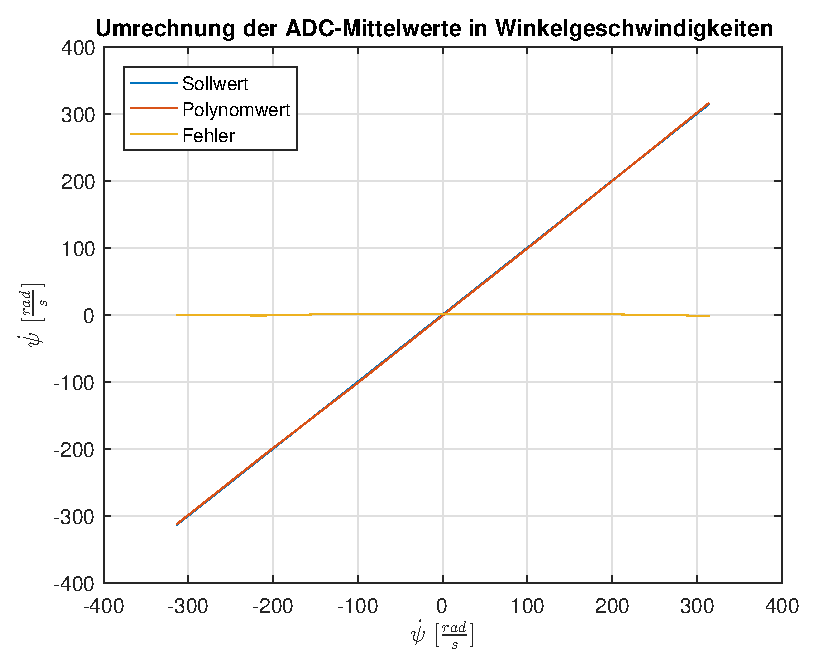
\includegraphics[width=0.5\linewidth]{img/ADC_mittelwert_polynom.eps}
\end{figure}

\subsection{Filterung der Sensordaten}
In der Regel werden Sensoren von Störungen unterschiedlichster Art beeinflusst. In diesem Abschnitt werden das Komplementär- und Kalman-Filter vorgestellt. Hierbei handelt es sich um Methoden der Datenfusion um möglicht präzise Schätzungen der Zustandsgrößen zu erreichen.

Der Ausfallwinkel $\varphi$ kann über die Auswertung der Beschleunigungswerte berechnet werden. Allerdings weißen diese Sensoren hochfrequente Störanteile auf, welche sich negativ auf die Winkelschätzung auswirken. Alternativ kann die Zustandsgröße $\varphi$ über die Integration der Winkelgeschwindigkeit $\dot{\varphi}$ gewonnen werden. Die Geschwindigkeit $\dot{\varphi}$ wird mit Hilfe der beiden Gyroskope gemessen. Allerdings sind diese Messungen von einer systematischen Messabweichung betroffen, welche in die Integration einfließt und somit zu einem langfristigen Drift des Winkels $\varphi$ führt.

\subsubsection{Komplementärfilter}
Eine der simpelsten Methoden der Signalverarbeitung stellt das s.g. Komplementärfilter dar. Die Grundidee dieses Prinzips besteht darin die einzelnen Sensorsignale mit einem Hoch- oder Tiefpass zu filtern und anschließend zu fusionieren. 

In diesem Anwendungsfall wird der Winkel $\varphi_{Acc}$, welcher über die Beschleunigungswerte berechnet wird, mit einem Tiefpass gefiltert. Dadurch werden die hochfrequenten Störsignale entfernt. Der zweite Winkelwert $\varphi_{Gyr}$, welcher durch die Integration der Winkelgeschwindigkeit $\dot{\varphi}$ gewonnen wird, kann mit Hilfe eines Hochpasses von dem niederfrequenten Störsignal befreit werden.

Dieses Fusionsprinzip führt zu den folgenden Berechnungsschritten.

\begin{enumerate}
 \item Integration der Winkelgeschwindigkeit $\dot{\varphi}_n$ nach der Trapezregel über das jeweilige Abtastintervall $t_a$.
 \begin{equation}
 \Delta \varphi_n = \frac{t_a}{2} \cdot (\dot{\varphi}_n + \dot{\varphi}_{n-1})
 \end{equation}
 \item Summation des vorherigen Winkels $\varphi_{n-1}$ mit der Winkeländerung $\Delta \varphi_{n}$.
 \begin{equation}
 \varphi_{Gyr,n} = \varphi_{n-1} + \Delta \varphi_{Int,n}
 \end{equation}
 \item Berechnung des aktuellen Winkels $\varphi_n$ mit einem gewählten Gewichtungsfaktor $\alpha$ und den Winkelschätzungen $\varphi_{Gyr,n}$ und $\varphi_{Acc,n}$.
 \begin{equation}
 \varphi_n = \alpha \cdot \varphi_{Gyr,n} + (1-\alpha) \cdot \varphi_{Acc,n}
 \end{equation}
\end{enumerate}

\subsubsection{Kalman-Filter}
Das Kalman-Filter beruht auf dem Prinzip der Zustandsschätzung. Diese Schätzung erfolgt mittels der Messwerte aus Gyroskopen, Beschleunigungssensoren und der darauf folgenden Winkelschätzung. Hierbei greift der Algorithmus auf Methoden der Wahrscheinlichkeitsrechnung zurück. Ist die Varianz eines Messfehlers gegeben, so kann eine Schätzung des tatsächlichen Zustandes vorgenommen werden.
In diesem Fall wird mit den linearisierten Bewegungsgleichungen gearbeitet. Dadurch kann das gewöhnliche Kalman-Filter verwendet werden. Für nichtlineare Systeme müssen unterschiedliche Filteralgorithmen, wie beispielsweise das Extended-Kalman-Filter, verwendet werden.


\begin{table}[h!]
\centering
\begin{tabularx}{0.9\textwidth}{|c|c|}
\hline
 \textbf{Bezeichnung}  	& \textbf{Erkärung} \\ \hline
 $\boldsymbol{x}^*_n$	&	Systemzustände \\ \hline
 $\hat{\boldsymbol{x}}_n$ & Geschätzte Systemzustände \\ \hline 
 $\boldsymbol{u}_n$		& 	Messbare Eingangsgrößen  \\ \hline
 $\boldsymbol{v}_n$		&	Störgrößen \\ \hline
 $\boldsymbol{A}_d$ 	& 	Systemmatrix, welche den Systemzustand $\hat{\boldsymbol{x}}_n$  \\  & auf den folgenden Zeitschritt abbildet. \\ \hline
 $\boldsymbol{B}_d$		&	Eingangsmatrix \\ \hline
 $\boldsymbol{C}_d$		&	Ausgangsmatrix \\ \hline
 $\boldsymbol{P}^*_n$	&	Kovarianzmatrix von $\boldsymbol{x}^*_n$. Legt die Sicherheit der Schätzung fest. \\ \hline
 $\hat{\boldsymbol{P}}_n$ & Filterkovarianzmatrix von $\hat{\boldsymbol{x}}_n$. Gibt die Gewichtung der Messwerte an. \\ \hline
 $\boldsymbol{Q}_n$		&	Kovarianzmatrix des Systemrauschens \\ \hline
 $\boldsymbol{R}_n$		& 	Kovarianzmatrix des Messrauschens \\ \hline
\end{tabularx}
\end{table}

Die Berechnung des Kalman-Filters verläuft in zwei Schritten, welche in insgesamt fünf Teile gegliedert ist. Zuerst wird der Prädikationsschritt durchgeführt, hierbei wird der Prädikationsschätzwert $\boldsymbol{x}^*_{n+1}$ berechnet, welcher den Systemzustand im folgenden Zeitschritt darstellt. Zusätzlich wird die Prädikationskovarianzmatrix $\boldsymbol{P}^*_{n+1}$ berechnet, welche angibt wie sicher die Vorhersage im Verhältnis zu dem wahren Systemzustand ist.
Im zweiten Abschnitt, der s.g. Korrektur- bzw. Filterschritt, wird die Vorhersage mit Hilfe der neuen Messwerte korrigiert. Hierfür wird zuerst die Verstärkungsmatrix $\boldsymbol{K_{n+1}}$ berechnet, welche den Rückkopplungsfaktor der Messwerte wiedergibt. Im Anschluss wird der Endschätzwertes des Systemzustandes mit Hilfe des ersten Prädikationswertes $\boldsymbol{x}^*_{n+1}$ und der Verstärkungsmatrix $\boldsymbol{K}_{n+1}$ bestimmt. Zuletzt wird die Varianz des geschätzten Systemzustandes $\hat{\boldsymbol{P}}_{n+1}$ berechnet.

\begin{enumerate}
	\item \textbf{Prädikationsschätzwert}
	\newline
	Der Systemzustand zum Zeitpunkt $n$ ist beschreibbar durch die zeitdiskrete, lineare, stochastische Differenzengleichung
	\begin{equation}
	\boldsymbol{x}^*_{n+1} = \boldsymbol{A}_d \cdot \boldsymbol{\hat{x}}_n + \boldsymbol{B} \cdot \boldsymbol{u}_n + \boldsymbol{v}_n
	\end{equation}
	Die Systemmatrix $\boldsymbol{A}$ bildet den Systemzustand $\boldsymbol{\hat{x}}$ von Zeitschritt $n$ auf den folgenden Zeitschritt $n+1$ ab. Die Eingangsgrößen $\boldsymbol{u}_n$ werden durch die Matrix $\boldsymbol{B}$ auf den Systemzustand $\boldsymbol{x}^*_{n+1}$ abgebildet. Das Rasuchen bzw. die äußeren Störeinflüsse werden durch den additiven Term $\boldsymbol{v}_n$ repräsentiert.
	\item \textbf{Prädikationskovarianzmatrix}
	\newline
	Die Kovarianzmatrix $\boldsymbol{P}^*_{n+1}$ gibt an, wie sicher die Prädikation im Verhältnis zu dem wahren Systemzustand ist.
	\begin{equation}
	\boldsymbol{P}^*_{n+1} = \boldsymbol{A} \cdot \boldsymbol{\hat{P}}_n \cdot \boldsymbol{A}^T + \boldsymbol{Q}_n
	\end{equation}
	\item \textbf{Verstärkungsmatrix} \newline
	Die Verstärkungsmatrix $\boldsymbol{K}_{n+1}$ wird für die Korrektur der Vorhersage verwendet. Sie bestimmt, mit welcher Verstärkung der Messvektor rückgekoppelt wird.
	\begin{equation}
	\boldsymbol{K}_{n+1} = (\boldsymbol{P}^*_{n+1} \cdot \boldsymbol{C}^T)(\boldsymbol{C} \cdot \boldsymbol{P}^*_{n+1} \cdot \boldsymbol{C}^T + \boldsymbol{R}_{n+1})^{-1}
	\end{equation}
	\item \textbf{Filterschätzwert}
	Mit Hilfe der Verstärkungsmatrix $\boldsymbol{K}_{n+1}$ und des Prädikationswertes $\boldsymbol{x}^*_{n+1}$ wird der finale Schätzwert des Systemzustandes zu dem Zeitpunkt $n+1$ bestimmt.
	\begin{equation}
	\boldsymbol{\hat{x}}_{n+1} = \boldsymbol{x}^*_{n+1} + \boldsymbol{K}_{n+1}(\boldsymbol{y}_{n+1} - \boldsymbol{C} \cdot \boldsymbol{x}^*_{n+1})
	\end{equation}
	\item \textbf{Filterkovarianzmatrix}
	Im letzten Schritt wird die Varianz des geschätzten Systemzustandes berechnet.
	\begin{equation}
	\boldsymbol{\hat{P}}_{n+1} = \boldsymbol{P}^*_{n+1} - \boldsymbol{K}_{n+1} \cdot \boldsymbol{C} \cdot \boldsymbol{P}^*_{n+1}
	\end{equation}
\end{enumerate}

\subsubsection{Anwendung des Kalman-Filters}
Um die zuvor angesprochenen Nachteile der einzelnen Sensoren auszugleichen, wird nun die Umsetzung eines Kalman-Filters zur Sensorfusion vorgestellt.

Das Kalman-Filter fusioniert den Ausfallwinkel $\varphi_{Acc}$ aus der Winkelschätzung mit der Winkeländerung $\Delta \varphi_{Gyr}$, welche durch Integration der Gyroskopwerte gewonnen wurde. Daraus ergibt sich der gefilterte Winkel $\hat{\varphi}_n$. Dieser gefilterte Zustandswert wird für die Berechnung des Regelkreises verwendet.

Als absolute Eingangsgrößen stehen hier zum einen die Winkelschätzung $\varphi_{Acc}$ und die Winkeländerung $\Delta \varphi_{Gyr}$ zur Verfügung. Somit kann das fehlerbehaftete Teilsystem durch folgende Gleichungen beschrieben werden, wobei $v_{Gyr,n}$ $w_{Acc,n}$ die störbehafteten Additionstherme darstellen.

\begin{equation}
\varphi_{n+1} = \varphi_{n} + \Delta \varphi_{Gyr,n} + v_{Gyr,n}
\end{equation}
\begin{equation}
\varphi_{Acc,n} = \varphi_n + w_{Acc,n}
\end{equation}


\newpage
\begin{figure}[h!]
\centering
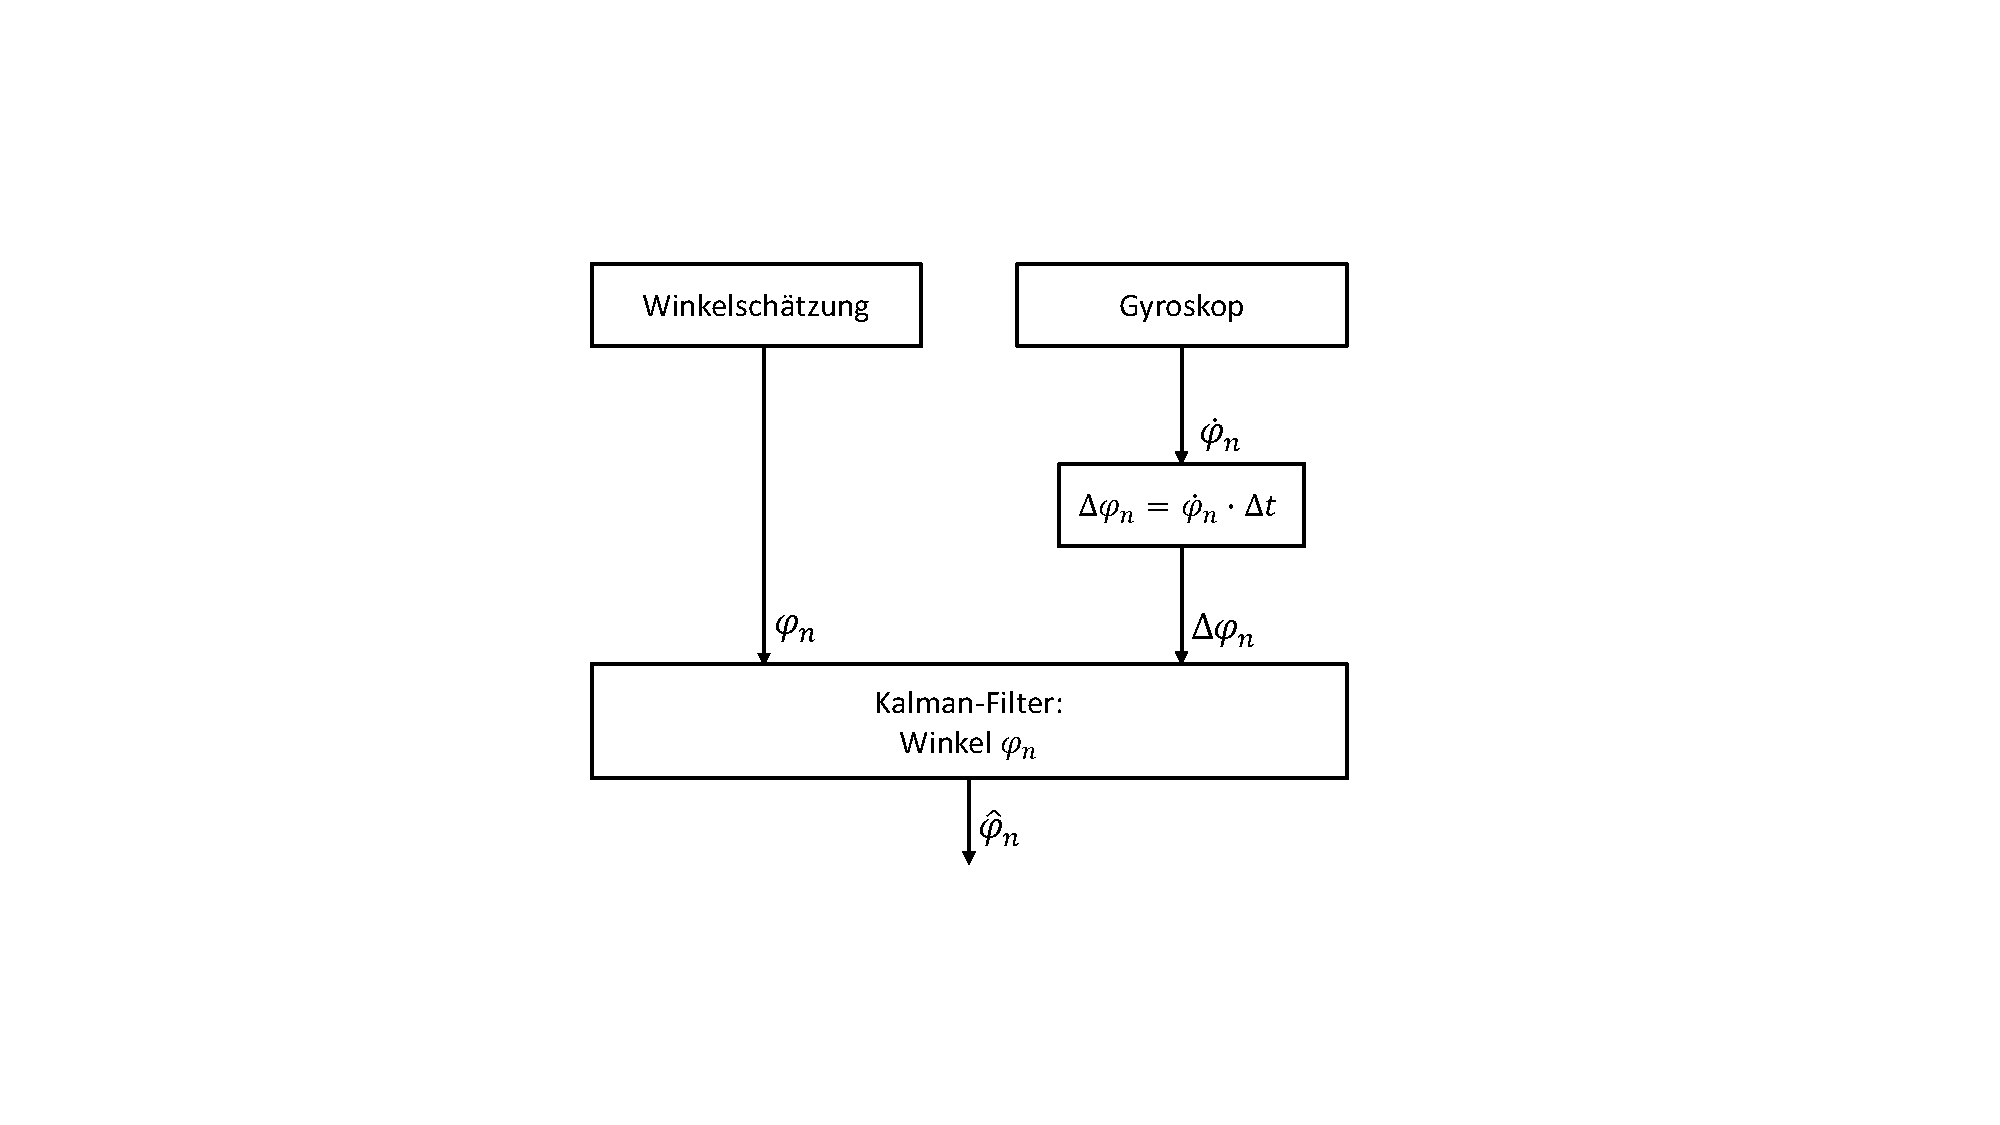
\includegraphics[width=\linewidth, trim={0 3.5cm 0 3.5cm},clip]{img/Kalman_overview}
\caption{Übersicht Kalman-Filter, Quelle: eigene Darstellung}
\end{figure}

Die bereits vorgestellten Berechnungsschritte können nun auf den spezifischen Anwendungsfall angepasst werden. Da lediglich eine einzelne Zustandsgröße berechnet wird, werden anstelle von Vektoren und Matrizen skalare Größen verwendet.

\begin{enumerate}
\item \textbf{Prädikationsschätzwert}
\begin{equation}
\varphi^*_{n+1} = \hat{\varphi}_n + \Delta \varphi_{Gyr,n}
\end{equation}
\item \textbf{Prädikationsvarianz}
\begin{equation}
P^*_{n+1} = \hat{P}_{n+1} + \sigma^2(\Delta \varphi_{Gyr,n})
\end{equation}
\item \textbf{Verstärkungsfaktor}
\begin{equation}
K_{n+1} = \frac{P^*_{n+1}}{P*_{n+1} + \sigma^2(\varphi_{Acc,n}}
\end{equation}
\item \textbf{Filterschätzwert}
\begin{equation}
\hat{\varphi}_{n+1} = \varphi^*_{n+1} + K_{n+1} \cdot (\varphi_{Acc,n} - \varphi^*_{n+1})
\end{equation}
\item \textbf{Filtervarianz}
\begin{equation}
\hat{P}_{n+1} = (1-K_{n+1}) \cdot P^*_{n+1}
\end{equation}
\end{enumerate}

\begin{figure}[h!]
\centering
\includegraphics[width=0.8\linewidth]{img/kalman_overview2}
\caption{Berechnungsablauf Kalman-Filter, Quelle: eigene Darstellung}
\end{figure}